\subsection{Verstellmechanik}
\label{verstellmechanik}
\textit{(ygu)} Die Hauptaufgabe der Verstellmechanik ist die automatisierte Einstellung aller geforderten Topfradien. Auch ist die Verstellmechanik Teil der Setzeinheit. Dabei kann keine klare Abgrenzung zur Setzeinheit gemacht werden, da in gewissen Komponenten Funktionen beider Einheiten vereint sind. Auch ist die Verstellmechanik klar als Wunschanforderung formuliert. Die Wunschanforderung birgt einen erhöhten Entwicklungsaufwand. Dieser Mehraufwand wird bewusst eingegangen, um ein Maximum an Automatisierungsgrad zu erreichen. Sollte trotzdem auf die automatische Verstellung der Topfradien verzichtet werden, ist die Entwicklung der Pflichtanforderung weniger zeitintensiv und rasch implementiert.
\newline

\subsubsection{Aufbau}
Die Konstruktion der Verstellmechanik basiert auf dem erstellten Funktionsmuster. Die Grundidee ist, dass über zwei Kulissen (eine radiale und eine lineare) der Topfradius zentral an einer Welle verstellt werden kann. Ein klarer Vorteil ist, dass dadurch nur ein Aktor für die Verstellung aller Stechdorne benötigt wird. Die Konstruktion kann in zwei Teile unterteilt werden:
\begin{itemize}
	\item \textbf{Bewegter Teil}: Dieser Teil wird durch die Spindel bewegt. Die drei Stechdorne (Punkt 4 in Abb. \ref{fig:details_vm}) sind durch zwei Kulissen (2, 3) verstellbar gelagert. Durch die Verbindung Keilnabe (5) - Keilwelle (1) sind diese mit dem unbewegten Teil gekoppelt. Eine geringes Gewicht des bewegten Teils ist für die Beschleunigung dieser Masse essentiell.
	
	\item \textbf{Unbewegter Teil:} Der unbewegte Teil dieser Einheit führt die Verstellung der Topfradien aus. Ein Getriebemotor (8), welcher durch eine Kupplung (9) mit der Keilwelle verbunden ist, führt die Verstellung der Topfradien aus. Diese Umsetzung besticht dadurch, dass anhand der Verbindung Keilnabe (5) - Keilwelle (1) bedeutend weniger Masse translatorisch beschleunigt wird. Dies bringt wertvolle Gewichteinsparnisse und wirkt sich positiv auf das benötigte Beschleunigungsdrehmoment M\textsubscript{a} aus.
\end{itemize}
	\begin{figure}[H]
	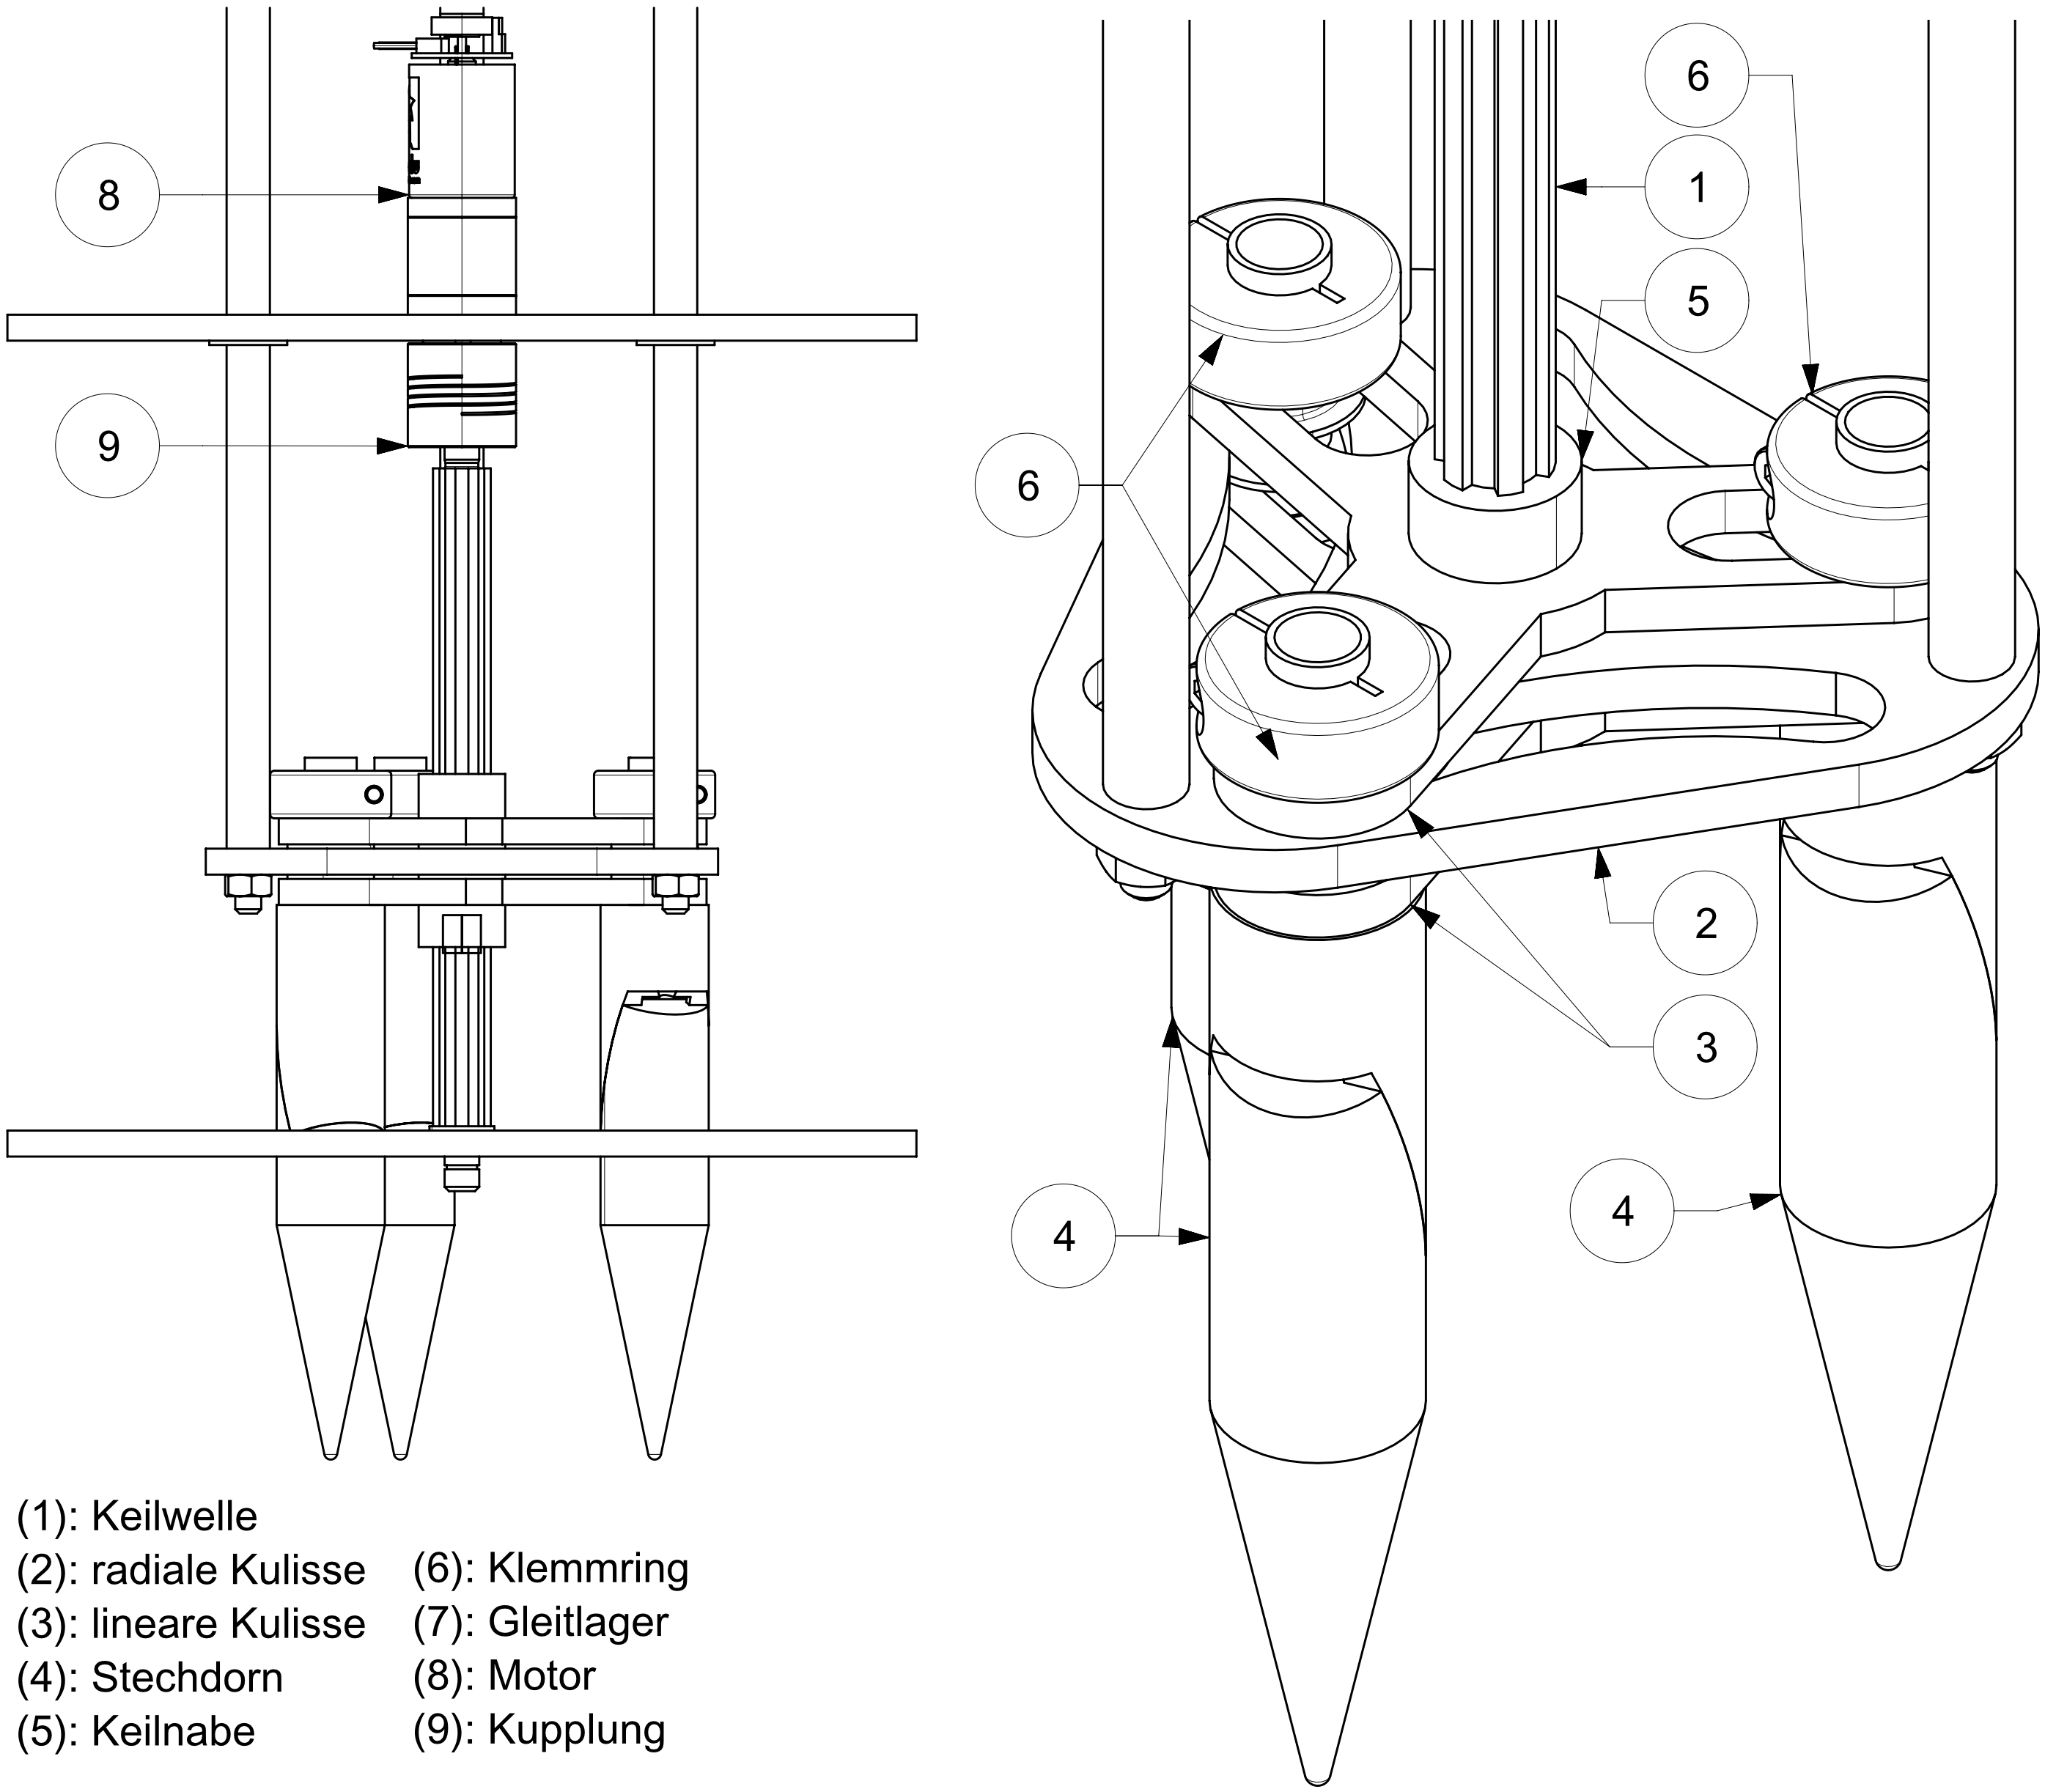
\includegraphics[scale=0.6]{Illustrationen/6-Umsetzung/details_vm.jpg}
	\caption{Detaillierte Übersicht der Verstellmechanik}
	\label{fig:details_vm}
	\end{figure}
Die Lagerung der Keilwelle wird nur wenig beansprucht, da durch die translatorische Freiheit der Keilnabe (entlang der Achse) keine Axialkräfte auftretten. Da die Verstellung des Topfradius nur wenige Male pro Tag vorgenommen wird, kann gemäss Roloff Matekk (Kapitel 14.3.1) von einer statischen Belastung (da n<10U/min) ausgegangen werden \cite{roloffmatek}. Daher ist die Verwendung eines Gleitlagers am unteren Ende (10) ausreichend. Verwendet wird das Gleitlager idlidur J3FM-0810 von Igus \cite{igusJ3FM}. Am oberen Ende ist die Keilwelle (1) über die Kupplung (9) durch den Getriebemotor (8) gelagert.
\newline

Der Stechdorn wird durch zwei lineare Kulissen (Punkt 3 in Abb \ref{fig:schnitt_vm}) und eine radiale Kulisse (2) geführt. Dabei sind die linearen Kulissen (3) mit der Keilnabe verbunden, die Radiale über die Führungen mit der Spindel. Um die Reibung zwischen Stechdorn und Kulissen zu vermindern werden auch hier Gleitlager (7) von igus eingesetzt. Die ganze Mechanik wird dabei durch die Auflage des Stechdorns (4) und einem Klemmring (6) gehalten.
	\begin{figure}[H]
	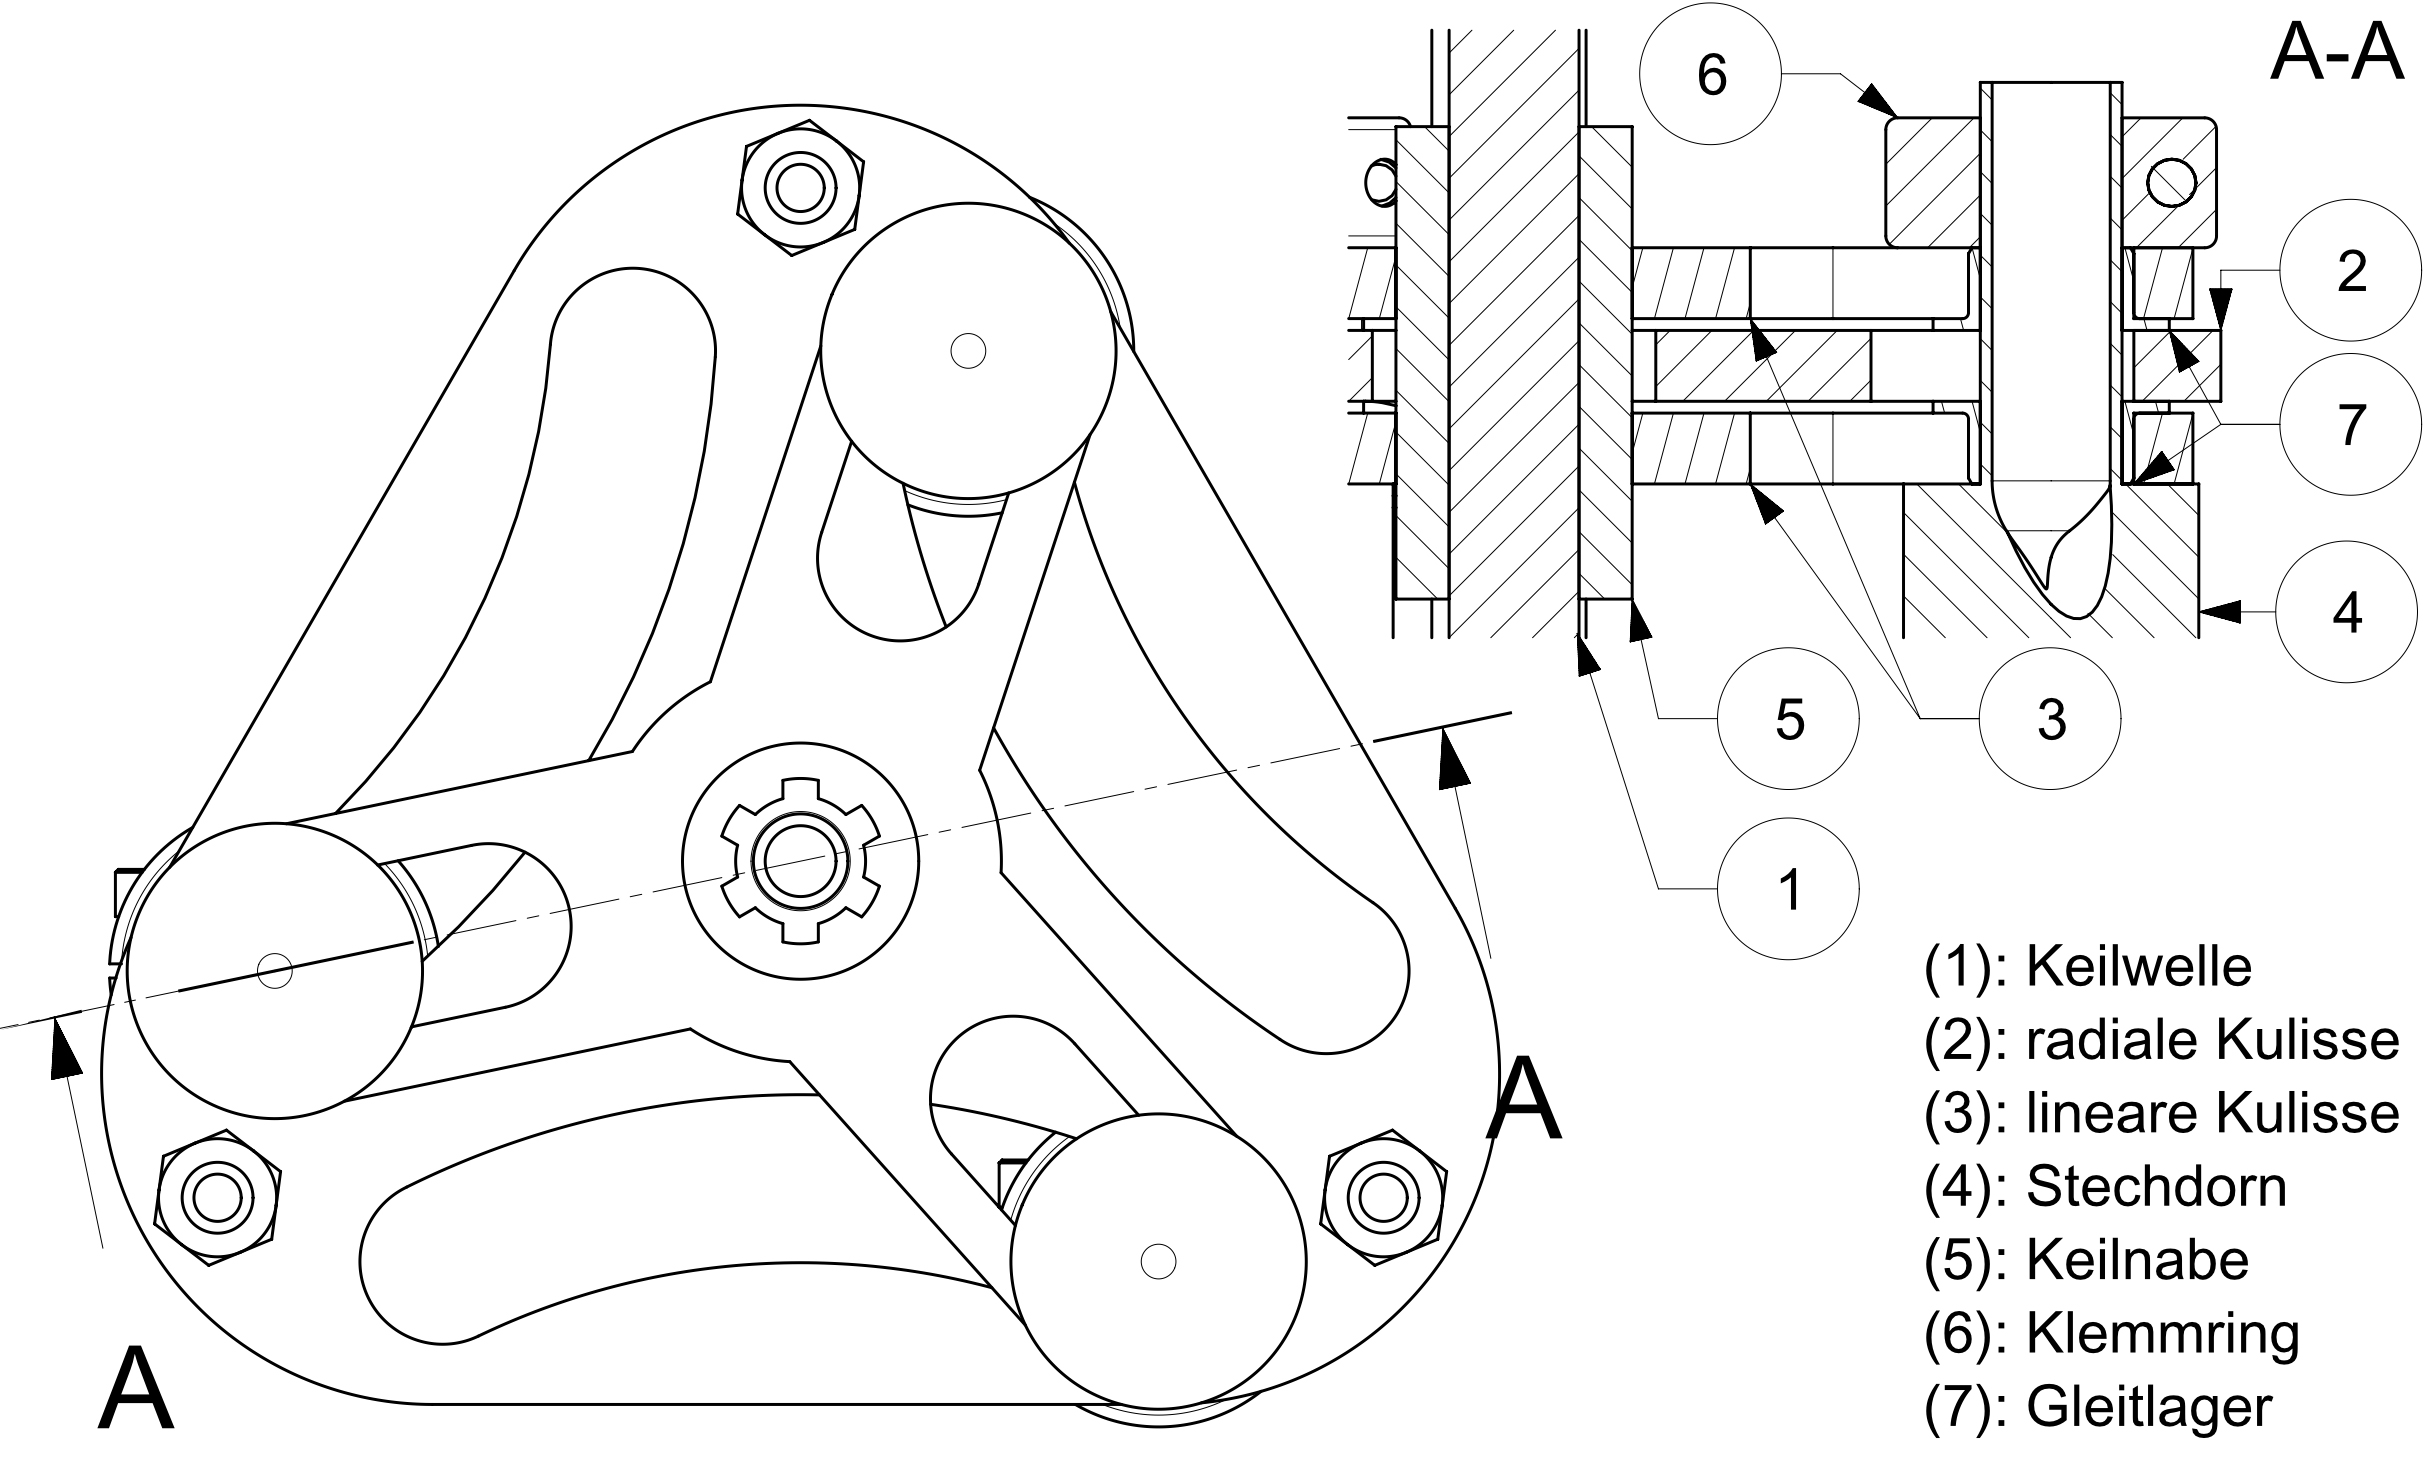
\includegraphics[scale=0.63]{Illustrationen/6-Umsetzung/schnitt_vm.jpg}
	\caption{Geschnittene Seitenansicht der Verstellmechanik}
	\label{fig:schnitt_vm}
	\end{figure}

\subsubsection{Funktion}
Die Bewegung der Verstellmechanik ist in Abbildung \ref{fig:motion_vm} dargestellt. Punkt B bildet ein beliebiger Punkt ab. Damit wird am Anschlag (Punkt A aus Abb. \ref{fig:motion_vm}) die Einsetzlokalität des grössten Topfes (Dmax = 140mm) und bei halbem Weg der Kulisse die Einsetzlokalität des kleinsten Topfes (Dmin = 90mm) erreicht. Dabei fällt auf, dass das Doppelte des nötigen Weges implementiert wurde. Begründet wird dies damit, dass dadurch der hochübersetzte Getriebemotor mehr Umdrehungen absolviert, bis der gewünschte Radius erreicht wird. Dies steigert die Auflösung des Motors und verbessert die Regelbarkeit.
	\begin{figure}[H]
	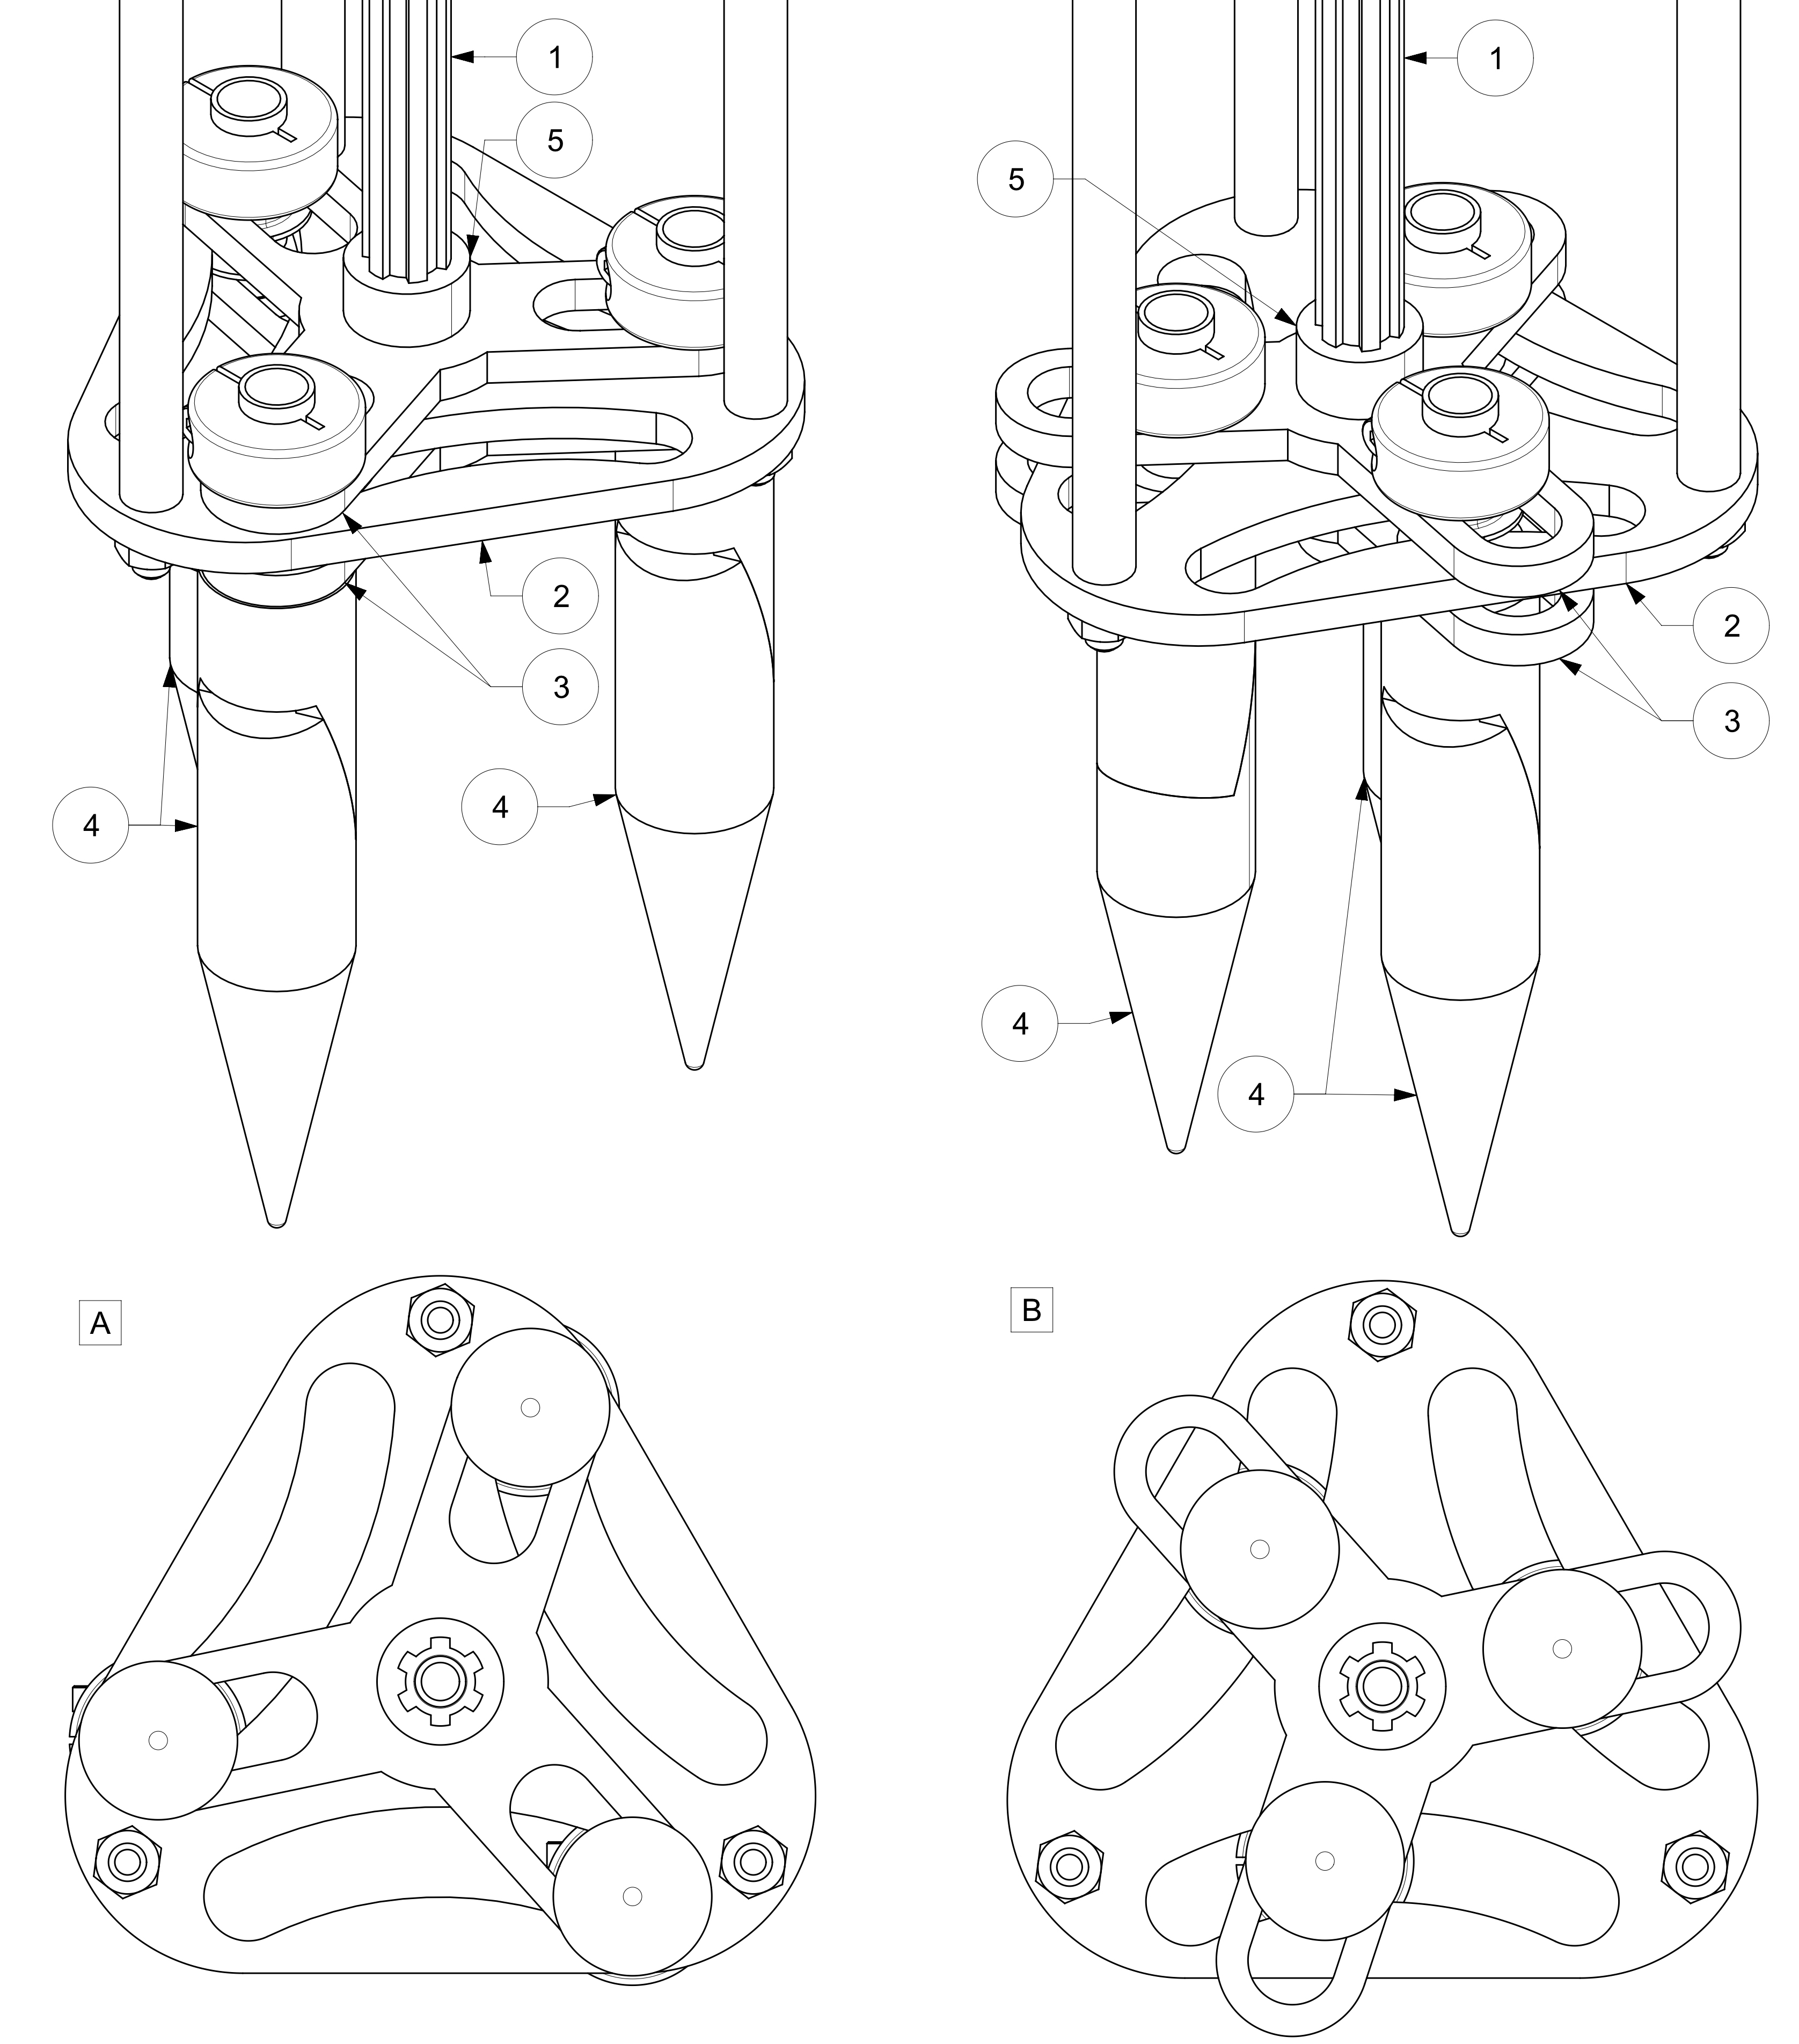
\includegraphics[scale=0.53]{Illustrationen/6-Umsetzung/motion_vm.jpg}
	\caption{Verstellung des Topfradius}
	\label{fig:motion_vm}
	\end{figure}
\subsubsection{Material und Fertigungsverfahren der Kulissen}
Wie schon erläutert, ist ein geringes Gewicht der beschleunigten Masse anzustreben. Gemäss Berechnungen soll die beschleunigte Masse maximal 1kg betragen. Um diese Anforderung zu erfüllen, werden die Kulissen (Punkte 2 und 3 aus Abb. \ref{fig:motion_vm}) aus 6mm dickem Aluminiumblech gefertigt. Auch die Teile werden mittels \textbf{Laserschneidmaschine} hergestellt. Weiter erspart diese Wahl das Umrüsten der Maschine und hält die Kosten auf einem Minimum (\textbf{nochmals nötig? Evtl. sinnvoller ein Kapitel 'Materialwahl' zu machen und einmal dafür ausführlich darauf eingehen}).